\subsection{Webanwendung}
\label{sec:webanwendung}
Frühere Webpräsenzen waren meist recht simpel gestaltet. Traditionell waren dies oft einfache Plattformen, um statische Informationen über das Internet zu verteilen. Einzig bei der Navigation durch die einzelnen Webseiten erfolgte eine Interaktion mit dem Besucher. Der Client schickt an den Webserver eine Anfrage, welche Webseite er gerne hätte, und erhält als Antwort das HTML-Dokument, siehe \autoref{img:http-website}.

\begin{figure}[H]
	\begin{center}

		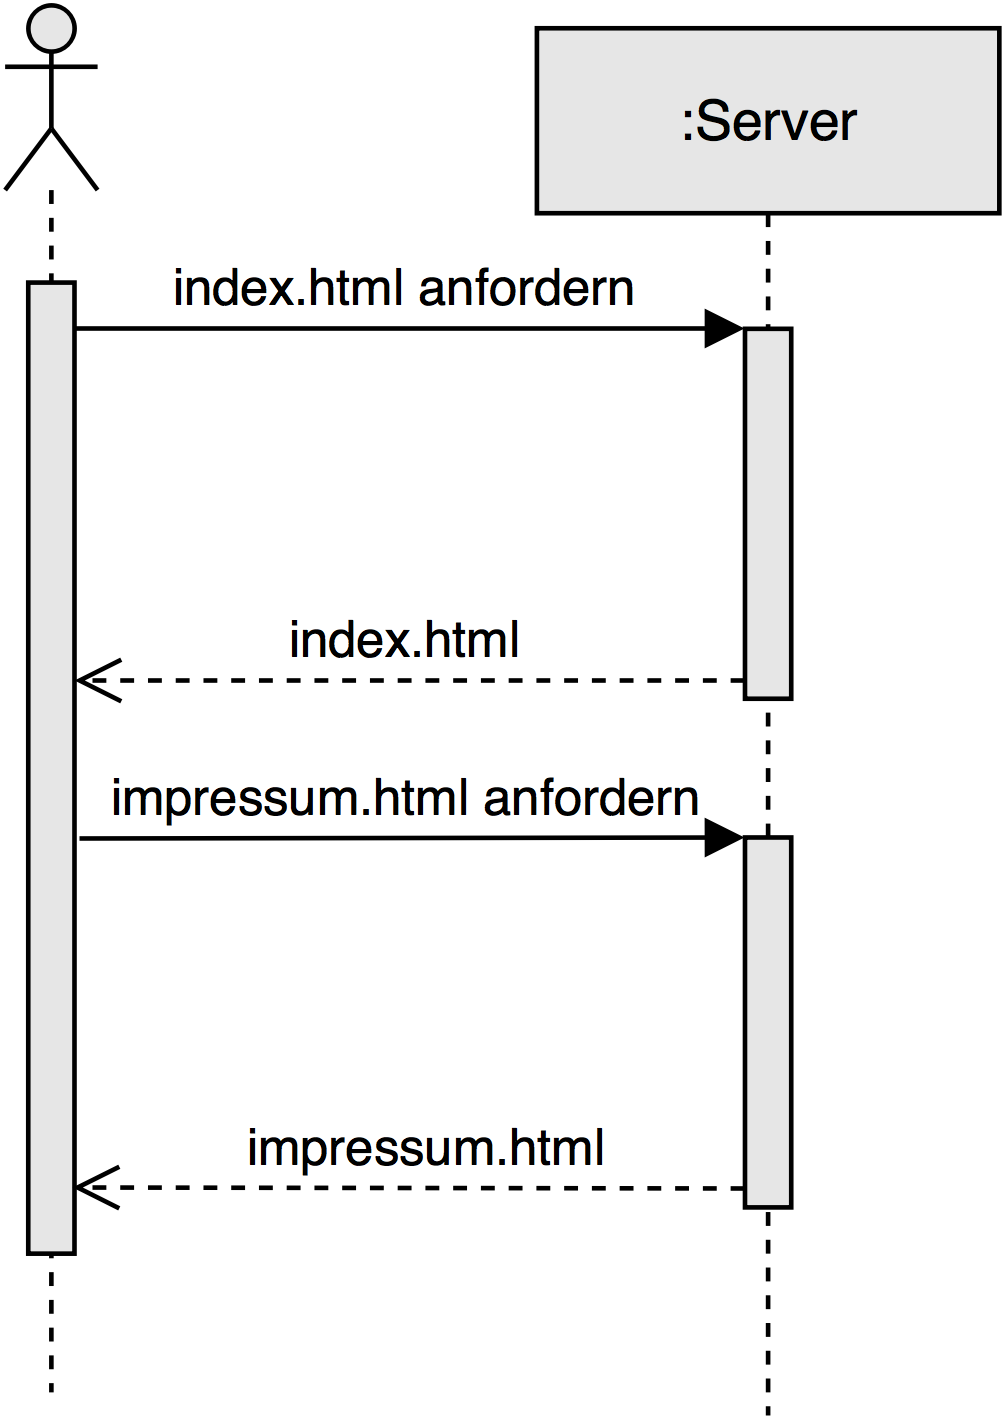
\includegraphics[width=.3\textwidth]{http-request.png}
		\caption{Systematischer Ablauf beim Abruf einer Webseite}
		\label{img:http-website}
	\end{center}
\end{figure}

Erst durch den Onlinehandel, webbasierte Buchungssysteme und Online-Auktionssysteme entstanden die ersten Webanwendungen als Weiterentwicklung von Webpräsenzen. Hierbei interagiert der Besucher neben der klassischen Navigation noch auf anderen Wegen mit der Webanwendung. So kann dieser zum Beispiel bei einem Onlinehändler für Musik durch die einzelnen Webseiten navigieren, durch entsprechende Anfragen das Musikangebot nach seinen Interessen filtern und Musikstücke erwerben \cite[S. 89]{lid00}. \\
Ein wesentlicher Unterschied zu Softwareanwendungen ist hier, dass eine Webanwendung mithilfe von Techniken und Standards, unter anderem vorgeschlagen vom \ac{w3c}, entwickelt wird und so Web-Ressourcen über einen Webbrowser bereitstellt \cite[S. 2]{kap03}.

\subsubsection{Serverseitige Webanwendungen}
\label{sec:server-webanwendung}

Für die Entwicklung von Webanwendungen wurden verschiedene Lösungsansätze entworfen. Diese lassen sich in erster Linie in serverseitige und clientseitige Lösungen einteilen.  \\
Bei serverseitigen Lösungen wird die Seite, abhängig von gewissen Parametern, vom Server zur Laufzeit generiert und an den Clienten gesendet. Als Beispiel soll ein Chatportal dienen. Dieses besteht aus einem Bereich für die Nachrichten, jeweils einem Feld für den Benutzernamen und die zu versendende Nachricht und einen Knopf zum Verschicken der Nachricht. Zur besseren Verdeutlichung dient \autoref{img:chat}.

\begin{figure}[H]
	\begin{center}
		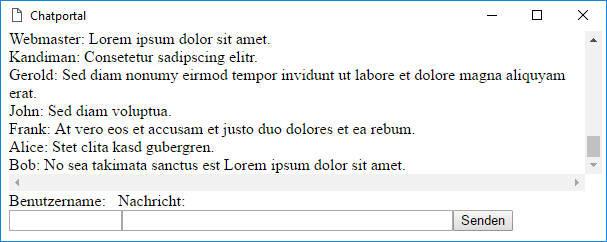
\includegraphics[width=.6\textwidth]{chat.png}
		\caption{Ein einfaches Beispiel eines Onlinechats}
		\label{img:chat}
	\end{center}
\end{figure}

Die serverseitige Lösung könnte vom Ablauf her in etwa wie in \autoref{img:webapp-server} aussehen.

\begin{figure}[H]
	\begin{center}
		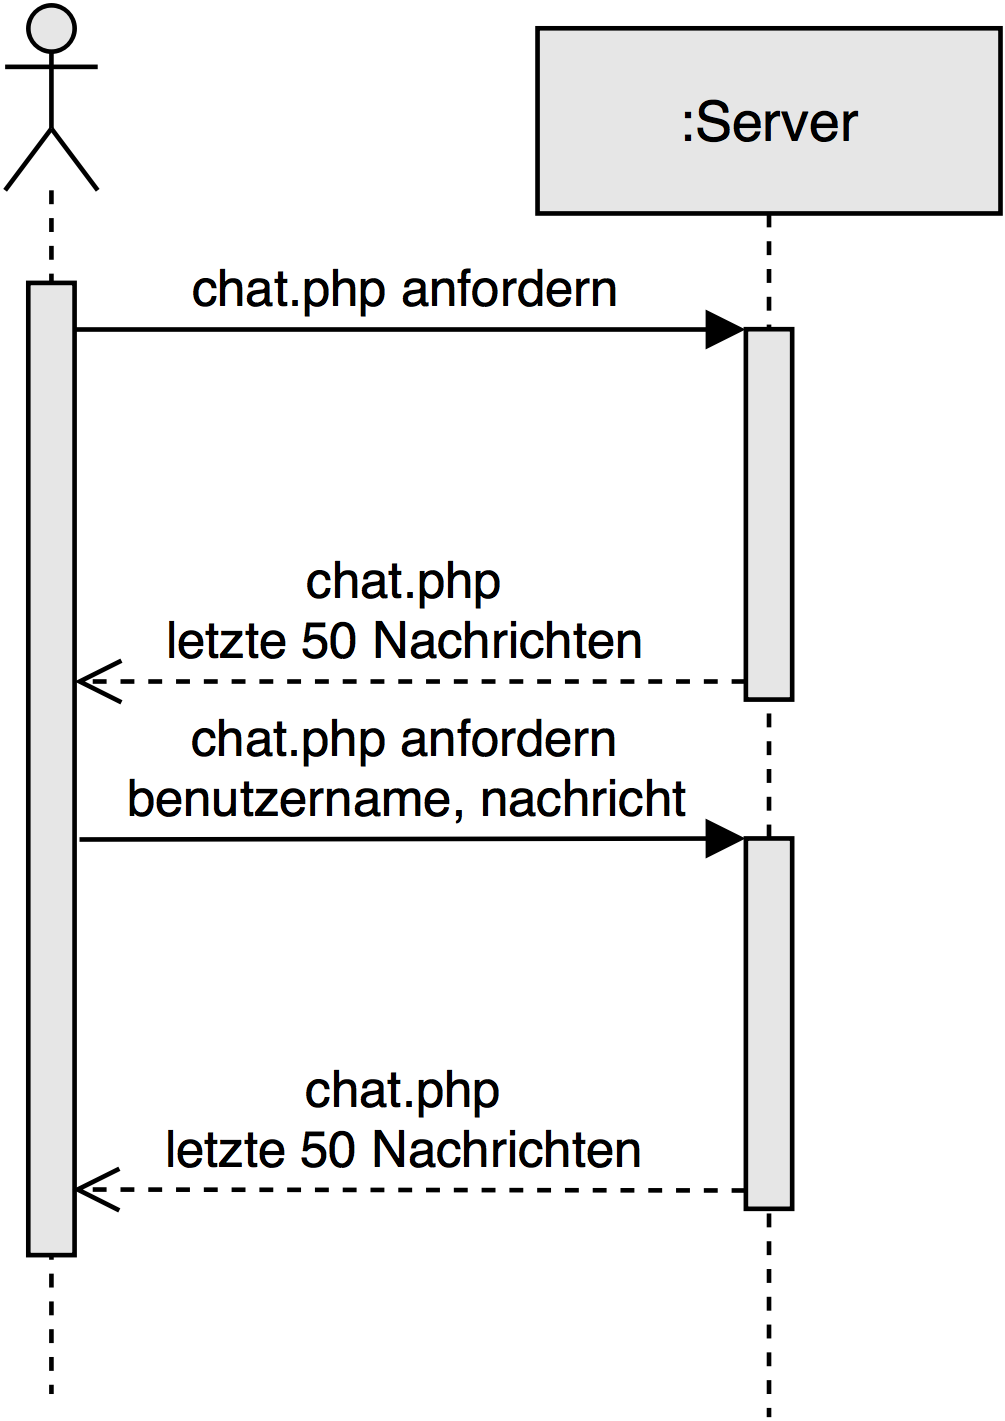
\includegraphics[width=.4\textwidth]{webapp-server.png}
		\caption{Kommunikation von Server und Client beim Laden neuer Informationen bei serverseitigen Webanwendungen}
		\label{img:webapp-server}
	\end{center}
\end{figure}


Bei der ersten Anfrage erhält der Benutzer die Webseite und die letzten 50 Nachrichten. Er kann die beiden Felder für den Benutzernamen und für die Nachricht befühlen und durch einen Klick auf die Schaltfläche \quotes{senden} beide Inhalte an den Server schicken. Dieser speichert die neue Nachricht samt dazugehörigen Namen und antwortet dem Clienten mit einer HTML-Seite, die alle neuen Nachrichten, seine eigene eingeschlossen, umfasst. Jede neue Nachricht führt hierbei zu einem kompletten Neuaufbau der Seite und einem erneuten Versenden der alten Nachrichten vom Server an den Clienten. Da auch die alten Nachrichten erneut mit versendet werden, hat dies einen erhöhten Datentransfer zur Folge.

\subsubsection{Clientseitige Webanwendungen}
\label{sec:client-webanwendung}

Um die Menge der zu versendenden Daten zu dezimieren, lassen sich clientseitige Lösungen zum Erstellen von Webanwendungen einsetzen. Diese bauen zumeist auf den Einsatz von JavaScript und Ajax. Die Nachrichten werden via Ajax an einen Service versandt und neue Nachrichten, ebenfalls mit Ajax, vom Service abgefragt. Neue und eigene Nachrichten werden durch DOM-Manipulation integriert, siehe \autoref{img:webapp-client}. 

\begin{figure}[H]
	\begin{center}
		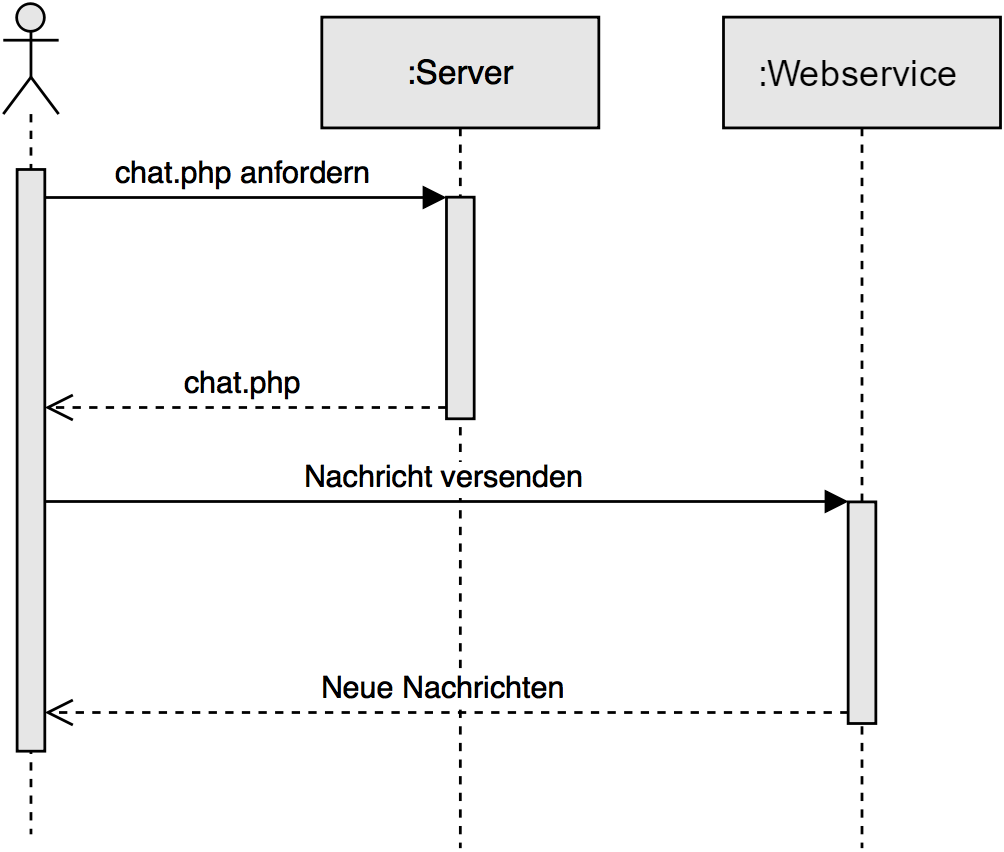
\includegraphics[width=.6\textwidth]{webapp-client.png}
		\caption{Kommunikation von Server und Client beim Laden neuer Informationen bei clientseitigen Webanwendungen}
		\label{img:webapp-client}
	\end{center}
\end{figure}

Ein Webservice\index{Webservice} ist hier ein Teil des Webservers, über den eine Maschine-zu-Maschine-Interaktion, typischerweise über HTTP, ermöglicht wird. Der Webservice besitzt eine vom Entwickler definierte Schnittstelle, über die der Austausch von Nachrichten ermöglicht wird.\\
Sowohl auf der Server- als auch auf der Clientseite wird der Datenverkehr verringert. Von Nachteil ist jedoch, dass im Browser auch JavaScript aktiviert sein muss. Ist dies nicht der Fall, so würde die Webanwendung nicht funktionieren. \\
\\
Beide Ansätze lassen sich auch kombinieren. So könnte das Chatportal bei seiner ersten Anfrage die alten Nachrichten abrufen. Alle neuen Nachrichten werden anschließend über Ajax nachgeladen.

\subsubsection{Single-Page-Webanwendung}
\label{sec:spa}

Durch den Einsatz von \ac{ajax} und \ac{dom} lässt sich auch eine \acf{spa} entwickeln. Diese werden im Deutschen auch Single-Page-Webanwendung genannt. Hierbei besteht eine Webpräsenz lediglich aus einer HTML-Seite, man täuscht dem Besucher aber bei der Navigation mehrere Webseiten vor \cite[S. 32]{ste15}. Dies wird erreicht, indem der Inhalt der neu anzuzeigenden Webseite durch Ajax geladen und durch DOM-Manipulation in die Seite integriert wird. Der alte Inhalt wird ausgeblendet und ist später, ohne dass eine weitere Ajax-Anfrage nötig ist, wieder eingeblendet. Durch Einsatz dieser Technik müssen auf den einzelnen Webseiten wiederkehrende Elemente, wie zum Beispiel Navigation, Kopf- und Fußzeilen etc. nur einmal zu Beginn geladen werden. Die Inhalte der bereits besuchten Seiten liegen weiterhin ausgeblendet beim Clienten vor und können relativ zügig durch DOM-Manipulation wieder eingeblendet werden. Analog zum Begriff Single Page Application werden klassische Webanwendungen, bei denen jeder Webseite eine HTML-Seite zugewiesen wird, auch \ac{mpa} genannt. Zu beachten ist, dass der Begriff \ac{mpa} in der Literatur nicht üblich ist und nur vereinzelt Verwendung findet. 